        %%******************************************%%
        %%                                          %%
        %%        Modello di tesi di laurea         %%
        %%            di Andrea Giraldin            %%
        %%                                          %%
        %%             2 novembre 2012              %%
        %%                                          %%
        %%******************************************%%

\begin{document}
    \frontmatter
    \input{preface/title-page}
    \input{preface/copyright}
    %\cleardoublepage
\phantomsection
\thispagestyle{empty}
\pdfbookmark{Dedica}{Dedica}

\vspace*{3cm}

\begin{center}
    Success is always stressful. \\ \medskip
    --- Andrew Tate
\end{center}

\medskip

% \begin{center}
    % Dedicated to myself
% \end{center}

    \cleardoublepage\phantomsection\pdfbookmark{Summary}{Summary}
\selectlanguage{english}
\begingroup
\let\clearpage\relax
\let\cleardoublepage\relax
\let\cleardoublepage\relax

\chapter*{Summary}
This document presents the outcomes of the internship conducted by Marco Bernardi at Breton S.p.A, spanning approximately three hundred hours. 
The internship encompassed various objectives, the first of which involved conducting a feasibility study on the utilization of Generative Adversarial Networks (GANs) for generating lifelike marble textures. 
Following the confirmation of feasibility, the subsequent goal was to develop a model capable of generating marble textures with a notable level of realism and diversity. 
Lastly, the final objective involved integrating the model into fundamental software designed for the creation of marble textures.

%\vfill

%\selectlanguage{english}
%\pdfbookmark{Abstract}{Abstract}
%\chapter*{Abstract}

%\selectlanguage{italian}

\endgroup

\vfill

    %\cleardoublepage
\phantomsection
\pdfbookmark{Acknowledgements}{acknowledgements}

\begin{flushright}{
    \slshape
    ``Life is really simple, but we insist on making it complicated''} \\
    \medskip
    --- Confucius
\end{flushright}


\bigskip

\begingroup
\let\clearpage\relax
\let\cleardoublepage\relax
\let\cleardoublepage\relax

\chapter*{Acknowledgements}

\noindent \textit{I want to thank \myProf, my thesis supervisor, for the support and patience he has shown me throughout my thesis.}\\

\noindent \textit{I would also like to thank my cat \textbf{mimì} for the support, the great help and for being close to me at all times during the years of study.}\\

\noindent \textit{Finally, thanks to all my economic supporters}\\

\bigskip

\noindent\textit{\myLocation, \myTime}
\hfill \myName

\endgroup

    \input{preface/table-of-contents}
    \cleardoublepage

    \mainmatter
    \chapter{Introduction}
\label{cap:Introduction}
% 
% Introduzione al contesto applicativo.\\
% 
% \noindent Esempio di citazione in linea \\
% \cite{site:agile-manifesto}. \\
% 
% \noindent Esempio di citazione nel pie' di pagina \\
% citazione\footcite{womak:lean-thinking} \\

\section{The company}

Breton S.p.A is an Italian company specializing in the manufacturing and engineering of high-tech machinery and systems for various industries. \\
Founded in 1963 by Marcello Toncelli, Breton has grown to become a global leader in the production of advanced industrial equipment. \\
The company's headquarters are located in Castello di Godego, Italy, 
and it operates multiple production facilities and subsidaries worldwide.\\
Breton is known for its cutting-edge technologies and innovative solutions, catering to sectors such as stone processing, metalworking, aerospace, automotive, and many more.
Breton's product portfolio encompasses a wide range of machinery, meeting the demands of both small-scale workshops and large industrial enterprises.\\
With a strong emphasis on research and development, Breton has made significant contributions to the advancement of automation and digitalization in various industries. The company continually invests in cutting-edge technologies, such as artificial intelligence, Internet of Things (\gls{iotg}), and machine learning, to provide state-of-the-art solutions to its customers.
Furthermore, Breton places a high value on sustainability and eco-friendly practices. The company focuses on developing energy-efficient machinery, reducing waste generation, and promoting sustainable manufacturing processes.
\subsection{Products and Services}
\subsubsection{Products}
Breton's product portfolio encompasses a wide range of machinery, including:
\begin{itemize}
    \item \textbf{CNC machines:} Breton's \gls{cncg} machines are designed to provide high precision and accuracy in machining operations. The company offers a wide range of CNC machines, including vertical machining centers, horizontal machining centers, and 5-axis machining centers.
    \item \textbf{Cutting and shaping systems:} Breton's cutting and shaping systems are designed to provide high precision and accuracy in cutting and shaping operations. The company offers a wide range of cutting and shaping systems, including waterjet cutting systems, laser cutting systems, plasma cutting systems, and wire cutting systems.
    \item \textbf{Polishing equipment:} Breton's polishing equipment is designed to provide high precision and accuracy in polishing operations. The company offers a wide range of polishing equipment, including polishing machines, polishing robots, and polishing systems.
    \item \textbf{Waterjet cutting systems:} Breton's waterjet cutting systems are designed to provide high precision and accuracy in waterjet cutting operations. The company offers a wide range of waterjet cutting systems, including waterjet cutting machines, waterjet cutting robots, and waterjet cutting systems.
    \item \textbf{Robotic solutions:} Breton's robotic solutions are designed to provide high precision and accuracy in robotic operations. The company offers a wide range of robotic solutions, including robotic arms, robotic cells, and robotic systems.
    \item \textbf{Software:} Breton provides software solutions for the management of the productivity process, that can be fully integrated with the existing systems, for grant the best performance of the machinery and grant the control over the production plant.
\end{itemize} 
\subsubsection{Services}
Breton offers a wide range of services to its customers, including:
\begin{itemize}
    \item \textbf{Consulting:} Breton provides consulting services to its customers, helping them choose the right machinery for their needs. The company's experts analyze the customer's requirements and recommend the most suitable solutions.
    \item \textbf{Installation:} Breton's technicians install the machinery at the customer's site and ensure that it is functioning properly.
    \item \textbf{Training:} Breton offers training programs to its customers, teaching them how to operate the machinery and get the most out of it.
    \item \textbf{Maintenance:} Breton provides maintenance services to its customers, ensuring that the machinery is running smoothly and efficiently.
\end{itemize}
\subsection{Certifications}
Breton is continuously improving its products, services and workflows to meet the highest standards of quality, safety, and environmental protection. \\
The company is certified according to the following standards:
\begin{itemize}
    \item \textbf{ISO 9001:} Breton is certified according to the ISO 9001 standard, which specifies requirements for a quality management system.
    \item \textbf{ISO 14001:} Breton is certified according to the ISO 14001 standard, which specifies requirements for an environmental management system.
    \item \textbf{UNI INAIL ed. 2001:} Breton is certified according to the UNI INAIL ed. 2001 standard, which specifies requirements for a health and safety management system.
\end{itemize}
\section{The idea}
The idea born from a company request, they want to extract the main features of a marble slab, such as the veins, texture, and colors for automatically create a digital fingerprint of the marble slab.\\
This digital fingerprint can be easily achieved with a classic \gls{mlg} model. Veins in marble slabs are not always the same, and the marble slabs are not always perfect, so teach to a \gls{mlg} model what is and what is not a veins could be very challenging.\\
For this reason it's needed a lot of images with the respective veins path for train the model, and this is not always possible for different reasons:
\begin{itemize}
    \item Breton work only on test slabs, so they don't have a large amount of images. 
    For solve this problem, they've to rely on the customers, and many times the customers don't want to share their images.
    \item Manually extract the veins path from the images is very time consuming, and will take a lot of time and human resources.
\end{itemize}
So the idea is to create a generative model that can generate a large amount of images with the respective veins path, and use this images for train the \gls{mlg} model.\\
\subsection{Side Idea}
From the main idea, born a side idea, that is to create a \gls{cncg} program from an image file.\\
In this way they can recreate veins on technological stones slabs, by the use of a \gls{cncg} machine.\\
This idea is very challenging, because convert an image file to a \gls{cncg} program is not a simple task, \gls{cncg} program is a list of instructions for the machine, and the image file is a matrix of pixels.\\
For this reason, the side idea was reverted and become: "Generate a marble slab image from a \gls{cadg} model".\\
The \gls{gang} model need to be able to reproduce colors, textures and the veins should follow the path of the \gls{cadg} model.\\
This is more feasible, the \gls{cadg} model can be easily converted to a \gls{cncg} program, and the \gls{cncg} program can be used for create a marble slab.\\

%% OLD IDEA
%The idea of the project was born from a request of some customers, that want to extract the main features of a marble slab, such as the veins, texture, and colors for creating a digital
%fingerprint of the marble slab.\\
%In this way the customer can have a digital copy of the marble slab, and can use it for create a \gls{cadg} model of the marble slab, and use it for create a \gls{cncg} program for the machines.\\
%Having a model capable of extract the main features of the marble slab, could reduce the workload of the designer, that can avoid to do it by hand.\\
%This request was a bit eulerian, because the veins are not always the same and the marble slab are not always perfect, so teach to a \gls{mlg} model what is and what is not a veins could be very challenging.\\
%Plus convert an image file to a \gls{cncg} program is not a simple task, because the \gls{cncg} program is a list of instructions for the machine, and the image is a matrix of pixels, so the conversion is not trivial.\\
%
%Then it was choose to revert the problem, and instead of convert an image to a \gls{cncg} program, it was choose to convert a \gls{cadg} file to an image, and the relative \gls{cncg} program.\\
%The \gls{gang} model need to be trained for reproduce the colors and the texture of the marble slab, with the given path of the veins exported from the \gls{cadg} file.\\
%This approach was more feasible, because the \gls{cadg} file can be easily converted to a \gls{cncg} program with the existing software.\\

\section{Objectives}
The objectives of the project could be classified in tree main categories recognized by the following letters:
\begin{itemize}
    \item \textbf{M:} Mandatory objectives, that are the main objectives of the project and a request of the commissioning company.
    \item \textbf{D:} Desiderable objectives, that are the secondary objectives of the project, not necessary
    for the commissioning company but that can give added value to the project.
    \item \textbf{O:} Optional objectives, that are the optional objectives of the project.
\end{itemize}
Each objectives can be identified by a unique code, that is composed by the letter of the category and a number that identify the objective.\\
The objectives are listed in the following table:

\begin{table}[H] 
    \caption{Mandatory objectives table}
    \label{tab:man-objectives}
    \centering
    \begin{tabularx}{\textwidth}{|c|X|c|}
        \hline
        \textbf{Code} & \textbf{Description} & \textbf{Category}\\
        \hline
        M1 & Get an analytic and multydisciplinar thought, thanks to the decomposition of the problem in subproblems & M\\
        \hline
        M2 & Reach a level of autonomy in the management of the project, with sinthesis and critical thinking of the problems & M\\
        \hline
        M3 & Quality on the production of technological artifacts and on the documentation & M\\
    \end{tabularx}
\end{table}

\begin{table}[H] 
    \caption{Desiderable objectives table}
    \label{tab:des-objectives}
    \centering
    \begin{tabularx}{\textwidth}{|c|X|c|}
        \hline
        \textbf{Code} & \textbf{Description} & \textbf{Category}\\
        \hline
        D1 & Development of a \gls{pocg} for generating marble images with a \gls{gang} model or similar technology & D\\
        \hline
        D2 & Development of a \gls{pocg} for augmenting resolution of an image & D\\
        \hline
        D3 & Validation of the artifacts produced & D\\
    \end{tabularx}
\end{table}

\begin{table}[H] 
    \caption{Optional objectives table}
    \label{tab:opt-objectives}
    \centering
    \begin{tabularx}{\textwidth}{|c|X|c|}
        \hline
        \textbf{Code} & \textbf{Description} & \textbf{Category}\\
        \hline
        O1 & First product engineering approaches developed & O\\
        \hline
        O2 & Product testing in a manufacturing production environment & O\\
    \end{tabularx}
\end{table}
\section{Text structure}

\begin{description}
    \item[{\hyperref[cap:Introduction]{First chapter}}] 
    The first chapter introduce the company and its products and services.\\
    It also describes the idea of the project and the text structure.

    \item[{\hyperref[cap:descrizione-stage]{Second chapter}}] The second chapter describes the process and the methodology used for the development of the project.
    
    \item[{\hyperref[cap:process-methodologies]{Third chapter}}] Third chapter describes the internship experience, in all its aspects.
    
    \item[{\hyperref[cap:design-coding]{Fifth chapter}}] The fifth chapter describes the design and the implementation of the project.
    It describes the technologies used and the architecture of the project.
    
\end{description}

During the writing of this document, the following conventions were adopted:
\begin{itemize}
    \item acronyms, abbreviations and ambiguous or uncommon terms mentioned are defined in the glossary, located at the end of this document;
    \item for the first occurrence of the terms defined in the glossary, the following nomenclature is used: \emph{word}\glsfirstoccur;
	\item the terms that require further explanation like technical words are marked with a subscript \emph{italic};
\end{itemize}

    \chapter{Process and methodologies}
\label{cap:process-methodologies}

\intro{Brevissima introduzione al capitolo}\\

\section{Evalutation of a GAN model}
\label{sec:evalutation-gan-model}
\subsection{The problem of evaluating GANs}
\label{subsec:problem-evaluating-gans}
Unlike other deep learning models, that are trained with a loss function until convergence, GANs are trained in a zero-sum game between two networks, the generator and the discriminator. 
The generator tries to fool the discriminator, while the discriminator tries to distinguish between real and fake samples. 
The training process is considered complete when the discriminator can no longer distinguish between real and fake samples. 
The generator is then considered to have learned the underlying distribution of the training data.\\
Thus, there is no objective function to minimize or maximize, and no way to objectively evaluate training progress and realtive or absolute performance of a GAN model from loss alone.
This is a major problem for GANs, when:
\begin{itemize}
    \item choosing a final GAN model during a training run;
    \item choosing generated samples to demonstrate the capabilities of a GAN model;
    \item comparing different GAN models;
    \item comparing different hyperparameters for the same GAN model;
\end{itemize}
So far, the most common way to evaluate GANs is to use a combination of qualitative and quantitative metrics based on the quality and diversity of the generated samples.
\subsection{Manual evaluation}
\label{subsec:manual-evaluation}
Many times the evaluation of a GAN model is done manually, by visual inspection of the generated samples.
This involves the use of human judgement to evaluate the quality of a batch of generated samples, and is therefore subjective.
Manual inspections is the simplest method of model evaluation, but it has many drawbacks:
\begin{itemize}
    \item it is subjective, including biases of the human evaluator about the model and the data;
    \item it require knowledge of the domain of the data;
    \item it is time consuming, so limited to the number of images that can be evaluated;
\end{itemize}
\emph{…evaluating the quality of generated images with human vision is expensive and cumbersome, biased […] difficult to reproduce, and does not fully reflect the capacity of models}
\footcite{paper:ganeval}.\\\\
This mean that this process will be for sure biased, so it shouldn't be used for a final model selection,
 but it can be used to get a first impression of the model performance.
Thankfully, more objective methods of evaluation have been proposed and adopted.
\subsection{Qualitative evaluation}
\label{subsec:qualitative-evaluation}
Qualitative measures are based on the visual inspection of the generated samples, but they are more objective than manual evaluation.
Some of the most common qualitative measures are:
\begin{itemize}
    \item \textbf{Nearest neighbors}: used to detect overfitting, by comparing the generated samples with the training data;
    \item \textbf{Rapid Scene Categorization}\footcite{paper:rapidscenecat}:in these experiments, subjects were asked to categorize images as real or fake as quickly as possible;
    \item \textbf{Rating and Preference judgement}\footcite{paper:stackadvnet}\footcite{paper:stackadvnet1}\footcite{paper:stackadvnet2}\footcite{paper:stackadvnet3}: 
    partecipants are asked to rate the quality of the generated samples, or to choose the best samples from a set of generated samples;
    \item \textbf{Mode Drop and Collapse}\footcite{paper:dropandcollapse}\footcite{paper:dropandcollapse2}: over datasets with multiple known modes, modes are coumputed as by measuring the distance of generated data to mode centers;
    \item \textbf{Network Internals}\footcite{paper:netint}\footcite{paper:netint1}\footcite{paper:netint2}\footcite{paper:netint3}\footcite{paper:netint4}\footcite{paper:netint5}: 
    the internal state of the models is used to evaluate the quality of the generated samples (e.g. space continuity, neuron activation, etc.);
\end{itemize}
The most used qualitative measure is a sort of manual inspection of images, called \emph{Rating and Preference judgement}.\\\\
\emph{These types of experiments ask subjects to rate models in terms of the fidelity of their generated images}\footcite{paper:ganeval}.\\\\
Usually images are shown in pairs (one real and one fake), and the subjects are asked to choose the best image.
A score or rating is then assigned to the model based on the number of times it is chosen as the best image.
For lowering the variance of the results, the images are shown to multiple human judges and the results are averaged.
This process is labor intensive, but with the help of crowdsourcing platforms like Amazon Mechanical Turk, 
it can be done at scale (Reducing the cost also).\\
Another downside of this method is that the human judges performance can improve with experience, especially if they are given feedback on their performance.\\\\
\emph{By learning from such feedback, annotators are better able to point out the flaws in generated images, giving a more pessimistic quality assessment}\footcite{paper:ganeval}.\\\\

Another similar method for subjectively evaluating the quality of generated images is \emph{"Nearest neighbors"}.
In this method, some examples of real images are picked from the domain of the data, and than it's picked the most similar generated images for comparison.
Some of the distance measures used for this method are Euclidean distance, cosine distance, and L1 distance.
Nearest neighbors can be used to determine how realistic the generated images are.


\subsection{Quantitative evaluation}
\label{subsec:quantitative-evaluation}
Quantitative measures are based on the use of metrics to evaluate the quality of the generated samples.
All this methods use a numerical score to evaluate the quality.
Some of the most common quantitative measures are:
\begin{itemize}
    \item Average log-likelihood;
    \item Coverage Metric;
    \item Inception Score;
    \item Modified Inception Score;
    \item Mode Score;
    \item AM Score;
    \item Frechet Inception Distance;
    \item Maximum Mean Discrepancy;
    \item The Wasserstein Distance;
    \item Birthday Paradox Test;
    \item Classifier Two-Sample Tests;
    \item Classification Performance
    \item Boundary Distortion 
    \item Number of Statistically-Different Bins
    \item Image Retrieval Performance
    \item Generative Adversarial Metric
    \item Tournament Win Rate
    \item Normalized Relative Discriminative Score
    \item Adversarial Accuracy and Adversarial Divergence
    \item Geometric Score
    \item Reconstruction Score
    \item Image Quality measures
    \item Low-level Image Statistics
    \item Precision, Recall and F1 Score
\end{itemize}

The most used quantitative measures are \emph{Inception Score} and \emph{Frechet Inception Distance}.
\subsubsection{Inception Score}
\label{subsubsec:inception-score}
Inception Score (IS) is a quantitative measure of the quality of generated images based on the Inception model.
It was proposed in 2016 by Tim Salimans et al. in \emph{"Improved Techniques for Training GANs"}\footcite{paper:salimans2016improved}.
The Inception Score is based on the idea that a good generative model should produce samples that are both \emph{diverse} and \emph{realistic}.
Calculating the IS requires the use of a pretrained Inception model, the Inception v3 model\footcite{paper:inceptionv3} and a dataset of generated images.
The Inception model is used to compute the conditional label distribution $p(y|x)$, where $x$ is an image and $y$ is a class label.
The Inception Score is then computed as:
\begin{equation}
    \label{eq:inception-score}
    \exp \left( \mathbb{E}_{x \sim p_{g}} \left[ \mathbb{KL}(p(y|x) || p(y)) \right] \right)
\end{equation}
where $p(y)$ is the marginal label distribution, and $p_{g}$ is the distribution of generated images.
The marginal label distribution $p(y)$ is approximated by computing the class distribution of the training set.
The Inception Score is then computed as the exponential of the KL divergence between the conditional label distribution and the marginal label distribution.
The KL divergence is a measure of how one probability distribution is different from a second, reference probability distribution.
The KL divergence is defined as:
\begin{equation}
    \label{eq:kl-divergence}
    \mathbb{KL}(p(y|x) || p(y)) = \sum_{y} p(y|x) \log \frac{p(y|x)}{p(y)}
\end{equation}
The Inception Score is a good measure of the quality of generated images, but it has some limitations.
The Inception Score is not a good measure of the diversity of generated images, and it is not a good measure of the quality of generated images when the dataset contains multiple modes.
\subsubsection{Frechet Inception Distance}
\label{subsubsec:frechet-inception-distance}
Frechet Inception Distance (FID) is a quantitative measure of the quality of generated images based on the Inception model.
It was proposed in 2017 by Martin Heusel et al. in \emph{"GANs Trained by a Two Time-Scale Update Rule Converge to a Local Nash Equilibrium"}\footcite{paper:heusel2017gans}.\\\\
\emph{"FID performs well in terms of discriminability, robustness and computational efficiency [...] It has been shown that FID is consistent with human judgments and is more robust to noise than IS".}\footcite{paper:ganeval}\\\\
Calculating the FID requires the use of a pretrained Inception model, the Inception v3 model\footcite{paper:inceptionv3} like the Inception Score.
The FID is computed as the Frechet distance between the feature representations of the real images and the generated images.
The Frechet distance is a measure of the similarity between two probability distributions.
The FID is defined as:
\begin{equation}
    \label{eq:frechet-inception-distance}
    \text{FID}(p_{r}, p_{g}) = \left\| \mu_{r} - \mu_{g} \right\|_{2}^{2} + \text{Tr} \left( \Sigma_{r} + \Sigma_{g} - 2 \left( \Sigma_{r} \Sigma_{g} \right)^{1/2} \right)
\end{equation}
where $\mu_{r}$ and $\mu_{g}$ are the mean vectors of the real and generated images, and $\Sigma_{r}$ and $\Sigma_{g}$ are the covariance matrices of the real and generated images.
The FID is a good measure of the quality of generated images, but it has some limitations.
The FID is not a good measure of the diversity of generated images, and it is not a good measure of the quality of generated images when the dataset contains multiple modes.
\subsubsection{Suggested GAN evaluation procedure}
\label{subsubsec:suggested-gan-evaluation-procedure}
At the starting of this section, we have seen that the evaluation of GANs is a difficult task.
A good way to evaluate GANs is to use a combination of qualitative and quantitative measures.
Starting with a manual inspection of the generated images, in order to evaluate the quality of the generator model.
After that, we can use some quantitative measures to evaluate the quality of the generated images and the diversity like the Inception Score and the Frechet Inception Distance.
Remember, that there is no single best measure for evaluating GANs, and that the choice of the evaluation measures depends on the task and the dataset.\\\\

\emph{
    As of yet, there is no consensus regarding the best score. Different scores assess various aspects of the image generation process, and it is unlikely that a single score can cover all aspects. Nevertheless, some measures seem more plausible than others (e.g. FID score)
}\footcite{paper:ganeval}\\\\
    \chapter{Internship description}\label{cap:internship-desc}
\intro{This chapter provides an overview of the internship project, including its requirements, goals, and the planning undertaken for the internship period.}
\section{Initial analysis}
The initial phase of the project involved an analysis of the requirements for developing a functional \gls{gang} model. 
This process entailed posing pertinent questions to determine the desired outcomes and the appropriate approach. 
These inquiries encompassed the nature of the generated images, the input image requirements, the network architecture, the extracted image features, and the dataset selection. 
By addressing these questions, the project's requirements, goals, and a comprehensive roadmap were established, laying the foundation for subsequent project execution.
%Given the idea of the project, the first step was to analyze the requirements for get a GAN model that was able to do the job.
%Some questions were made to understand what we want to achieve and how to do it.
%\begin{itemize}
%    \item\textbf{What kind of images the model should generate?}
%    \item\textbf{What kind of images the model should receive as input?}
%    \item\textbf{What kind of network should be used?}
%    \item\textbf{What kind of features should be extracted from the images?}
%    \item\textbf{What kind of dataset should be used?}
%\end{itemize}
%From the previous questions, was possible to define Requirements, Goals and a road-map for the project.\\
\section{Requirements \& Goals}
\subsection{Requirements}
\begin{itemize}
    \item \textbf{Requirement 1}: The dataset used for training the \gls{gang} model must consist of high-quality images of marble slabs to ensure accurate representation;
    \item \textbf{Requirement 2}: The model should possess the capability to generate realistic marble slab images based on given inputs, such as sketches or other forms of guidance;
    \item \textbf{Requirement 3}: The generated images produced by the model should exhibit a high level of quality, comparable to real images of marble slabs, in terms of visual fidelity, texture, and details;
    \item \textbf{Requirement 4}: The generated images should be presented in real time, allowing for immediate visual feedback and preview during the image generation process.
\end{itemize}
\subsection{Goals}
\begin{itemize}
    \item \textbf{Goal 1}: Acquire a diverse and high-quality dataset of marble slab images that encompasses various patterns, colors, and textures to train the \gls{gang} model effectively;
    \item \textbf{Goal 2}: Develop a \gls{gang} model that demonstrates the ability to generate accurate and visually appealing marble slab images from provided inputs, such as sketches or other relevant data;
    \item \textbf{Goal 3}: Create a desktop application that employs the trained \gls{gang} model to generate marble slab images in real time, enabling users to preview the generated images promptly during the image generation process. 
    This application should provide an intuitive user interface for seamless interaction.
\end{itemize}
\section{Planning}
Initially, the project was planned using a story map (See fig.~\ref*{label:story-map}) to define the main features of the project and the main steps to achieve them.
\begin{figure}[H]
    \centering
    \includegraphics[width=1\textwidth]{images/story-map.jpg}
    \caption{Story map}\label{label:story-map}
\end{figure}
\subsection{Road-map}
Following an initial analysis of the story map, it was feasible to establish a project roadmap encompassing the requirements and objectives to be accomplished during the internship period. 
The entire undertaking has been meticulously planned, employing a distinct temporal division across various phases. 
These phases are outlined below:
\begin{itemize}
    \item \textbf{Train period}: This phase entails an in-depth study of the current state of the art and the technologies that will be employed;
    \item \textbf{First period}:  During this phase, the focus will be on image acquisition;
    \item \textbf{Second period}: The primary objective of this period is to augment the dataset by increasing the number of images;
    \item \textbf{Third period}:  In this phase, the key task is to extract the main features;
    \item \textbf{Fourth period}: Network training constitutes the central objective of this Internship;
    \item \textbf{Fifth period}: The final phase involves the analysis of results and the implementation of improvements;
\end{itemize}
%After an Initial analysis of the story map, was possible to define a road-map for the project based on requirements and goals to achieve in the Internship period.
%All the activity has been planned using a specific division of the time in different phases.
%\begin{itemize}
%    \item \textbf{Train period}: study of the state of the art and the technologies that will be used;
%    \item \textbf{First period}: images acquisition;
%    \item \textbf{Second period}: dataset increase, images augmentation;
%    \item \textbf{Third period}: main feature extraction;
%    \item \textbf{Fourth period}: network training;
%    \item \textbf{Fifth period}: results analysis and improvement;
%\end{itemize}
\begin{landscape}
\begin{ganttchart}[%Specs
    y unit title=0.5cm,
    y unit chart=0.6cm,
    x unit=1.0cm,
    vgrid,hgrid,
    title height=1,
%     title/.style={fill=none},
    title label font=\bfseries\footnotesize,
    bar/.style={fill=blue},
    bar height=0.7,
%   progress label text={},
    group right shift=0,
    group top shift=0.7,
    group height=.3,
    group peaks width={0.2},
    inline]{1}{12}
   %labels
   \gantttitle{Internship Project}{12}\\  % title 1           
   \gantttitle{April}{4}                      % title 3
   \gantttitle{May}{4}
   \gantttitle{June}{4}
   % Setting group if any
   \ganttgroup[inline=false]{Train Period}{2}{3}\\ 
   \ganttbar[progress=100,inline=false]{Technology exploration}{2}{3}\\

   \ganttgroup[inline=false]{First Period}{3}{4}\\ 
   \ganttbar[progress=100,inline=false]{Image acquisition}{3}{4}\\
   \ganttmilestone[inline=false]{Milestone 1}{4} \\

   \ganttgroup[inline=false]{Second Period}{3}{4}\\ 
   \ganttbar[progress=100,inline=false]{Dataset improvements}{3}{4}\\
   \ganttmilestone[inline=false]{Milestone 2}{4} \\

   \ganttgroup[inline=false]{Third Period}{4}{5}\\ 
   \ganttbar[progress=100,inline=false]{Features extraction}{4}{5}\\
   \ganttmilestone[inline=false]{Milestone 3}{5} \\

   \ganttgroup[inline=false]{Fourth Period}{5}{7}\\ 
   \ganttbar[progress=100,inline=false]{Network training}{5}{7}\\
   \ganttmilestone[inline=false]{Milestone 4}{7} \\

   \ganttgroup[inline=false]{Fifth Period}{7}{11}\\ 
   \ganttbar[progress=50,inline=false]{General improvements \& Docs}{7}{11}\\
   \ganttmilestone[inline=false]{Milestone 5}{11} \\
\end{ganttchart}
\end{landscape}
\subsection{Study Period:}
This designated period was allocated for an in-depth examination of the current state of the art and the technologies that would be employed throughout the course of the internship. 
The primary focus areas encompassed the following key topics:
\begin{itemize}
    \item \textbf{Machine Learning}: A comprehensive study of the fundamental concepts and principles underpinning machine learning and deep learning;
    \item \textbf{\gls{gang}}: An extensive exploration of the core concepts and functioning principles of GANs;
    \item \textbf{GAN applications}: An examination of the principal applications of \gls{gang}s and their practical utilization;
    \item \textbf{GAN architectures}: A detailed analysis of the primary \gls{gang} architectures and their respective applications;
    \item \textbf{GAN training}: A thorough investigation into the predominant techniques employed for training \gls{gang}s;\@
    \item \textbf{GAN evaluation}: An in-depth exploration of the leading methodologies utilized for evaluating the performance of \gls{gang}s;\@
    \item \textbf{GAN improvements}: A comprehensive study of the key techniques employed to enhance and refine \gls{gang} models;\@
    \item \textbf{GAN applications}:  An exploration of the primary domains where \gls{gang}s find application and their practical implementation;
\end{itemize}
\subsection{First Period:}
During this designated period, the focus was on acquiring images. 
Each Breton machine was already equipped with a camera and a computer featuring specialized software capable of capturing images from the camera. 
The camera captured photographs of each worked slab, which were then transmitted to the database. 
Subsequently, the images were retrieved from the database and stored in a designated folder.
\subsubsection{Challenges:}
The primary challenge encountered during this phase pertained to the quality of the acquired images. 
The machine's image acquisition functionality was not originally intended for use in a machine learning project, resulting in suboptimal image quality. 
The images displayed variations in size, inconsistent backgrounds, and occasionally contained unwanted elements such as light reflections or machine shadows.
\subsubsection{Solutions:}
TTo address these challenges, the following measures were implemented:
\begin{itemize}
    \item \textbf{Background Removal}: To eliminate extraneous elements from the images, a pre-trained machine learning model developed by Breton was employed. 
    This model, in conjunction with the OpenCV library, effectively identified and removed non-slab components from the images, focusing solely on the slabs themselves.
    \item \textbf{Image Defects}: Manual intervention was employed to remove images with light reflections and shadows from the dataset. 
    This task was feasible due to the manageable quantity of such images.
    \item \textbf{Images Resizing}: The images were resized to a standardized dimension while preserving the original aspect ratio.
\end{itemize}
\subsubsection{Milestone:}
At the conclusion of this period, the dataset consisted of 500 images of slabs (See fig.~\ref{fig:slab-sample}), featuring diverse colors and textures. 
The dataset was subsequently divided into two separate parts: one for training purposes and the other for validation, with a split ratio of 70\% for training and 30\% for validation, respectively.
\begin{figure}
    \centering
    \includegraphics[height=6cm]{slabs/intera}
    \caption{Example of a slab}\label{fig:slab-sample}
\end{figure}

\subsection{Second Period:}
During this designated period, the dataset was expanded, and the existing images underwent augmentation techniques.
\subsubsection{Image Augmentation:}
Image augmentation is a technique employed to increase the number of images in a dataset by applying various transformations to the original images. 
This technique proves valuable when the dataset size is insufficient to train a network effectively.
To expand the dataset, each original image was split into smaller images of dimensions 256$\times$256 pixels (See fig.~\ref{fig:slab-split}).
After that the following augmentation techniques were applied to the images:
\begin{itemize}
    \item  \textbf{Resize}: Each image was resized to a larger dimension, increasing from 256$\times$256 pixels to 286$\times$286 pixels;
    \item  \textbf{Random Crop}: A random cropping operation was performed on each image, resulting in a standardized size of 256$\times$256 pixels;
    \item  \textbf{Random Flip}: Each image underwent a random horizontal flipping operation;
\end{itemize}
\subsubsection{Milestone:}
Upon the conclusion of this period, the dataset comprised 7000 images of slabs, exhibiting diverse colors and textures.

\begin{figure}
    \centering
    \includegraphics[width=.24\textwidth]{slabs/crop/crop_0_0}
    \includegraphics[width=.24\textwidth]{slabs/crop/crop_0_1}\\
    \vspace{0.1cm}
    \includegraphics[width=.24\textwidth]{slabs/crop/crop_1_0}
    \includegraphics[width=.24\textwidth]{slabs/crop/crop_1_1}
    \caption{Cropped image}\label{fig:slab-split}
\end{figure}

\subsection{Third Period:}
This designated period was dedicated to identifying the optimal method for extracting features from the images, such as veins, textures, and colors. 
The extraction of features from the images is a critical aspect of the project, as the quality of these features directly impacts the quality of the network. 
Thus, it was imperative to ensure the accuracy of the mask containing the extracted features.

\subsubsection{Vein Extraction:}
Various Python-implemented methods were tested for vein extraction. 
The tested methods included:
\begin{itemize}
    \item \textbf{Thresholding}\footcite{site:opencv-threshold}: This method utilizes the Threshold algorithm, which applies a threshold to the image, retaining only the pixels with values higher than the threshold. 
    To account for varying light conditions across images, the threshold was calculated using the Otsu's method.
    \item \textbf{Canny Edge Detection}\footcite{site:opencv-canny}: This method employs the Canny algorithm, which is an edge detection algorithm utilizing a multi-stage approach to identify edges in images. 
    The algorithm comprises five steps: noise reduction through Gaussian filtering, gradient calculation, non-maximum suppression, double thresholding, and edge tracking by hysteresis. 
    Figure~\ref{fig:canny_compare} illustrates the outcome of Canny Edge Detection
    \begin{figure}[H]
        \centering
        \includegraphics[width=.7\textwidth]{slabs/canny/canny}
        \\
        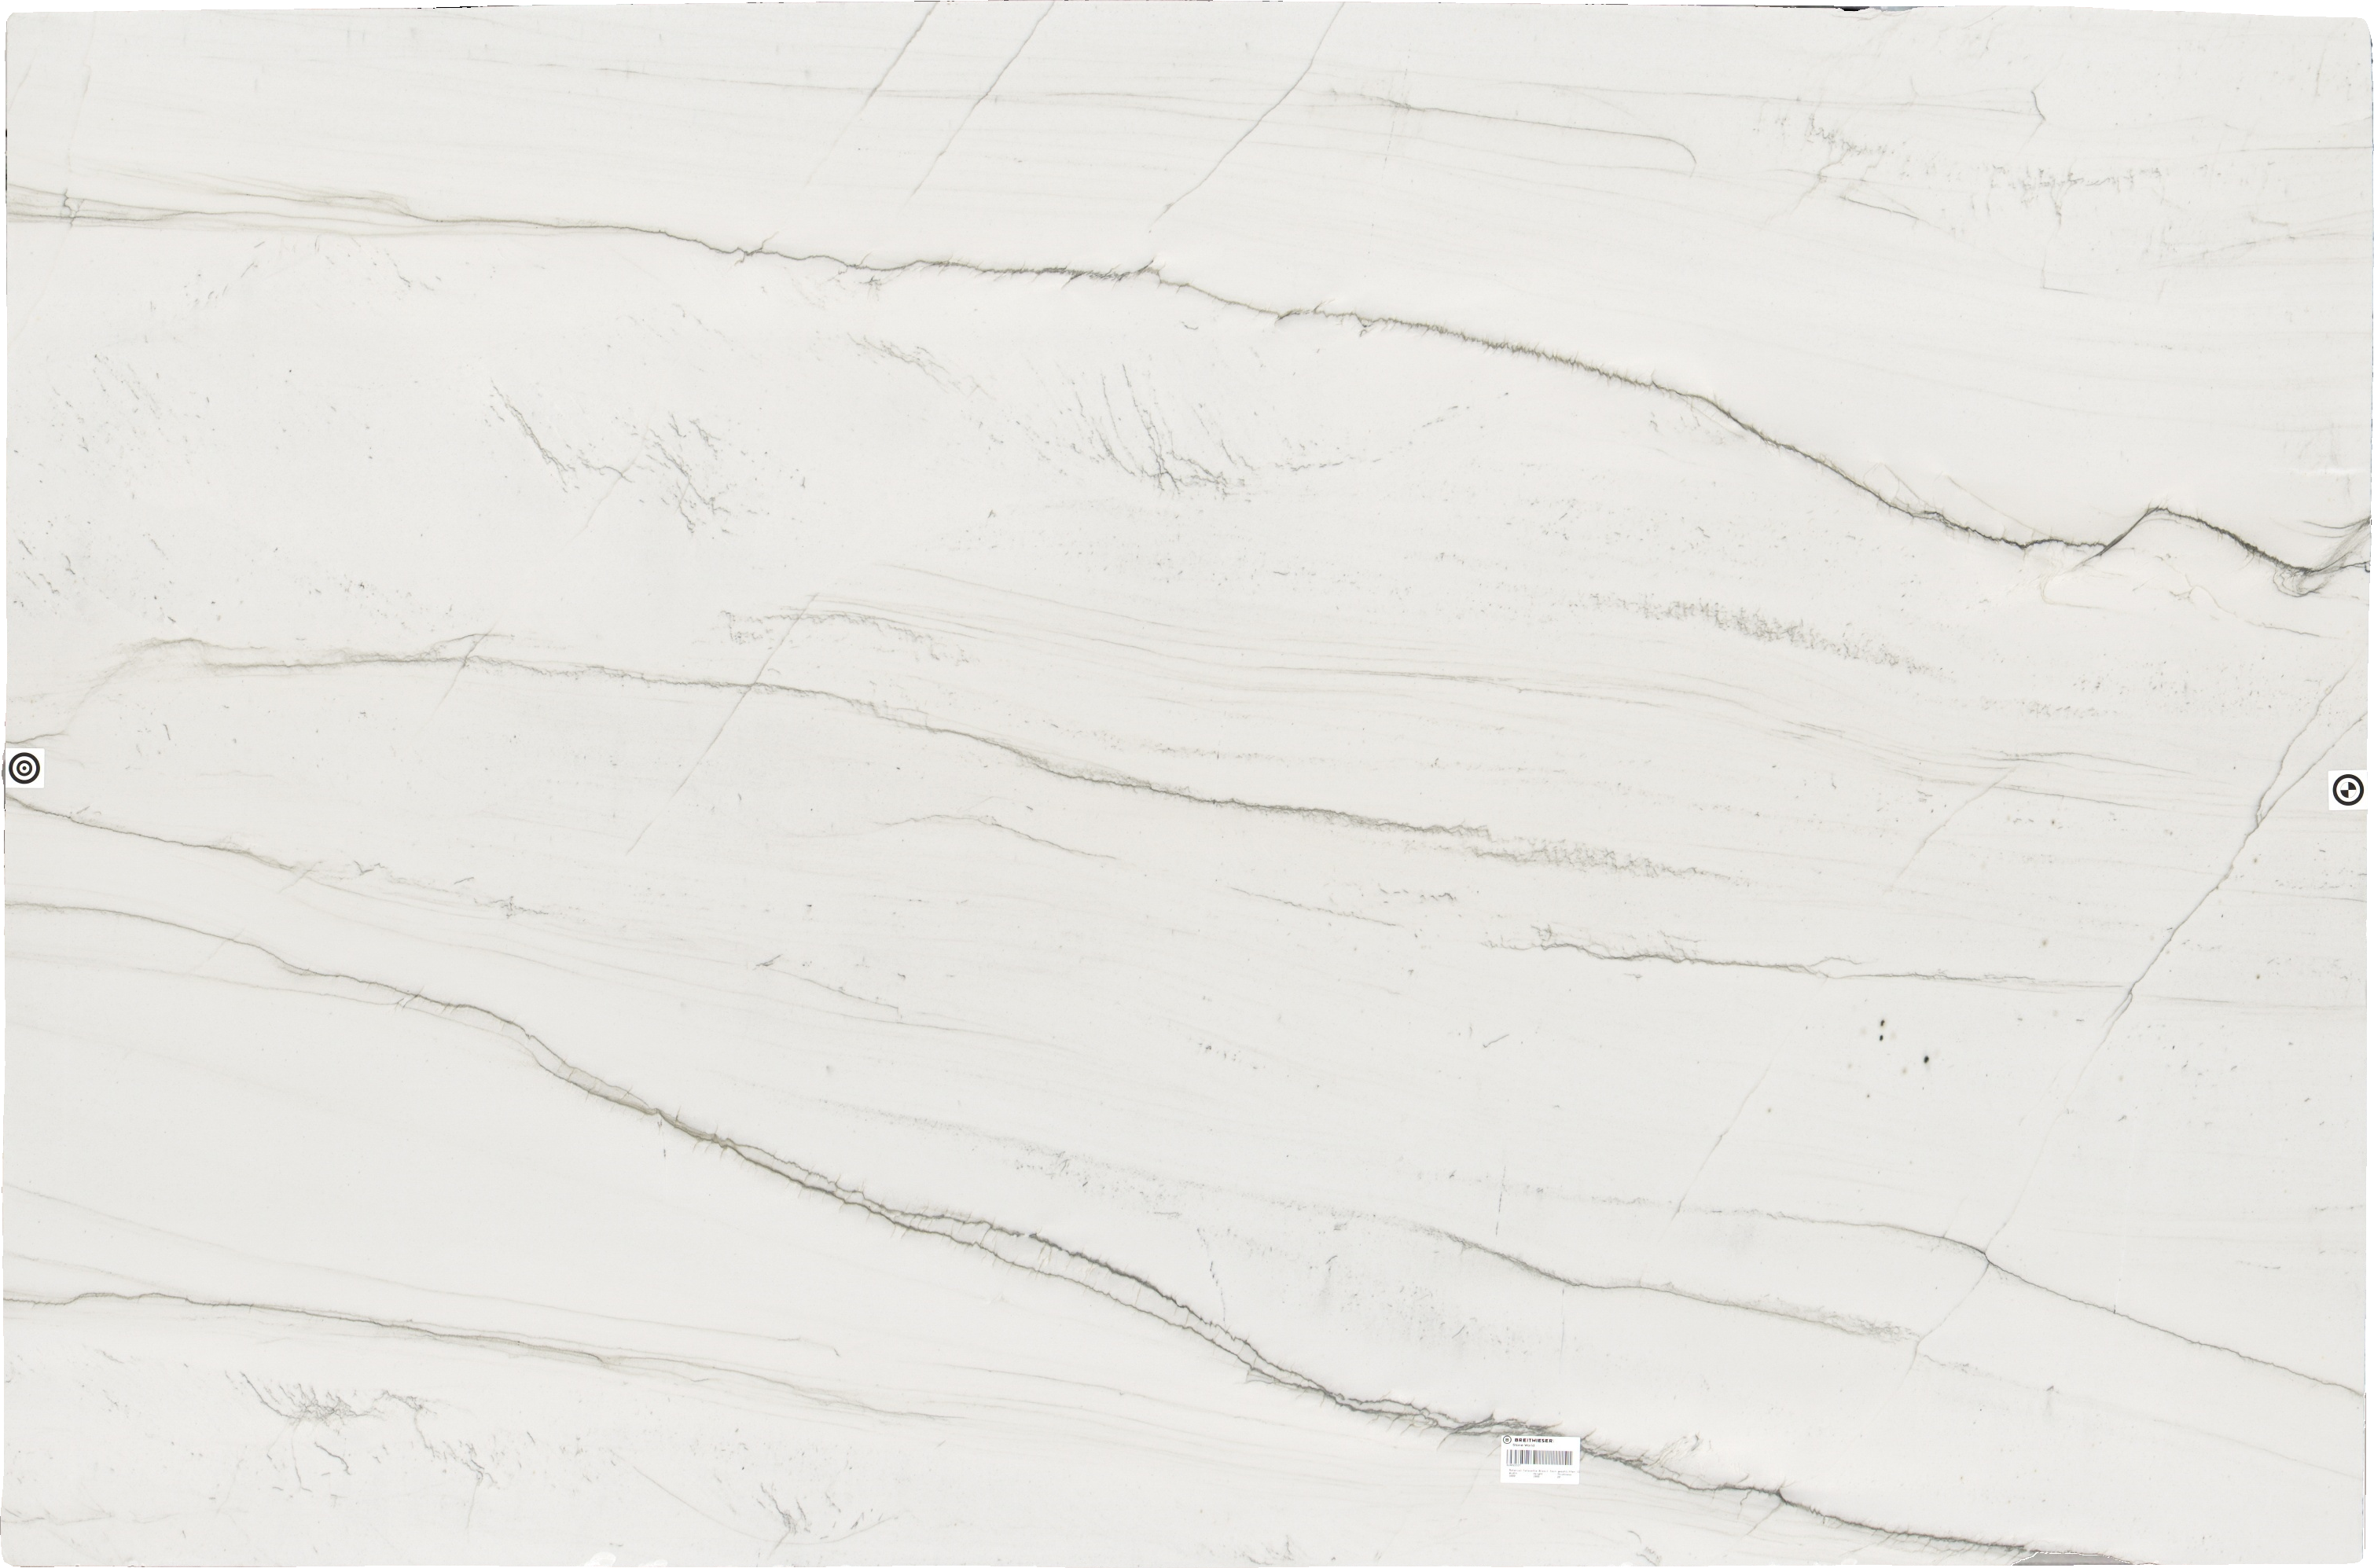
\includegraphics[width=.7\textwidth]{slabs/canny/canny_origin}
        \caption{Canny Edge Detection}\label{fig:canny_compare}
    \end{figure}
    \item \textbf{Meijering \& Contrast filter}\footcite{site:sckit-meijering}: The Meijering filter is based on the Hessian matrix, which calculates the second-order partial derivatives of a function. 
    Eigenvalues and eigenvectors obtained from the Hessian matrix enable the identification of line-like structures in the image. 
    The contrast filter is employed to enhance image contrast. 
    Figure~\ref{fig:meij_compare} presents the result of the Meijering \& Contrast filter.
    \begin{figure}[H]
        \centering
        \includegraphics[width=.7\textwidth]{slabs/meijering/meije}
        \\
        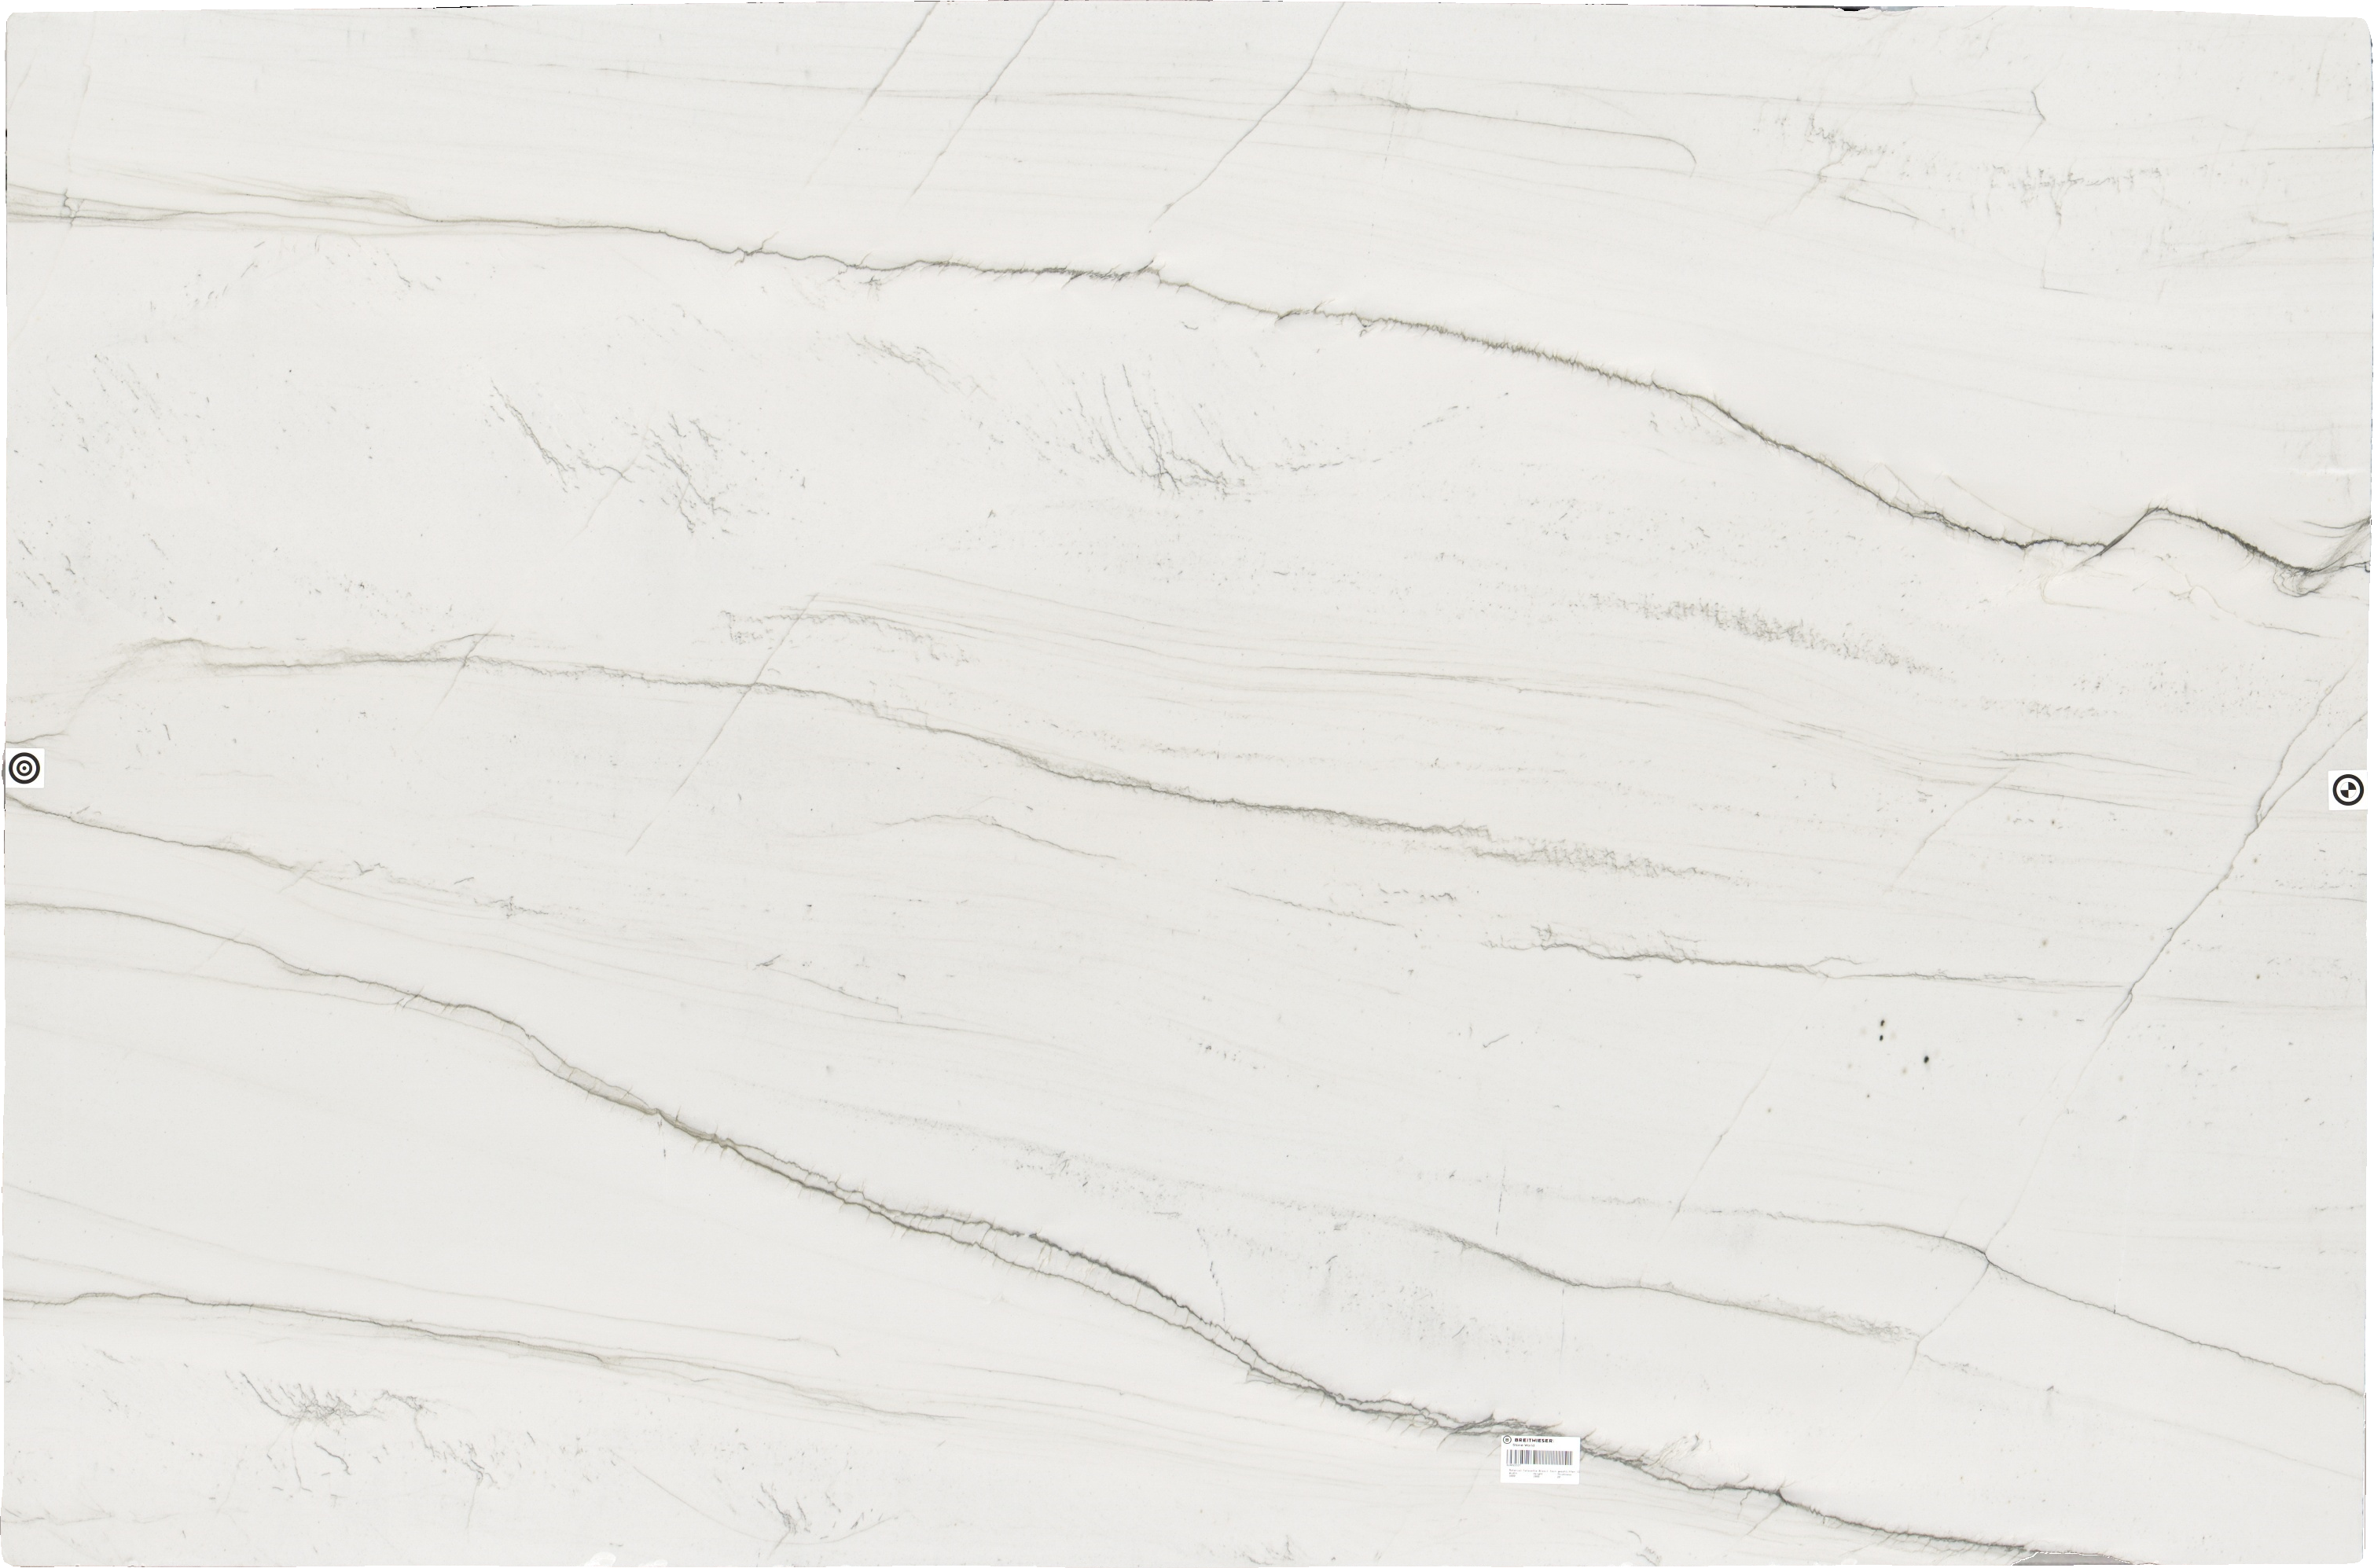
\includegraphics[width=.7\textwidth]{slabs/canny/canny_origin}
        \caption{Meijering \& Contrast filter}\label{fig:meij_compare}
    \end{figure}
    \item \textbf{HED (Holistically-Nested Edge Detection)}\footcite{paper:hed}: This method is based on the \gls{HEDG}\glsfirstoccur algorithm, which employs a deep neural network for edge detection in images. 
    The algorithm involves three steps: utilizing a pre-trained network to extract features from the image, applying a multi-scale algorithm to extract edges from the features, and linking the edges using the Canny algorithm. 
    Figure~\ref{fig:hed_compare} showcases the result of the \gls{HEDG} algorithm.
    \begin{figure}[H]
        \centering
        \includegraphics[width=.7\textwidth]{slabs/hed/hed}
        \\
        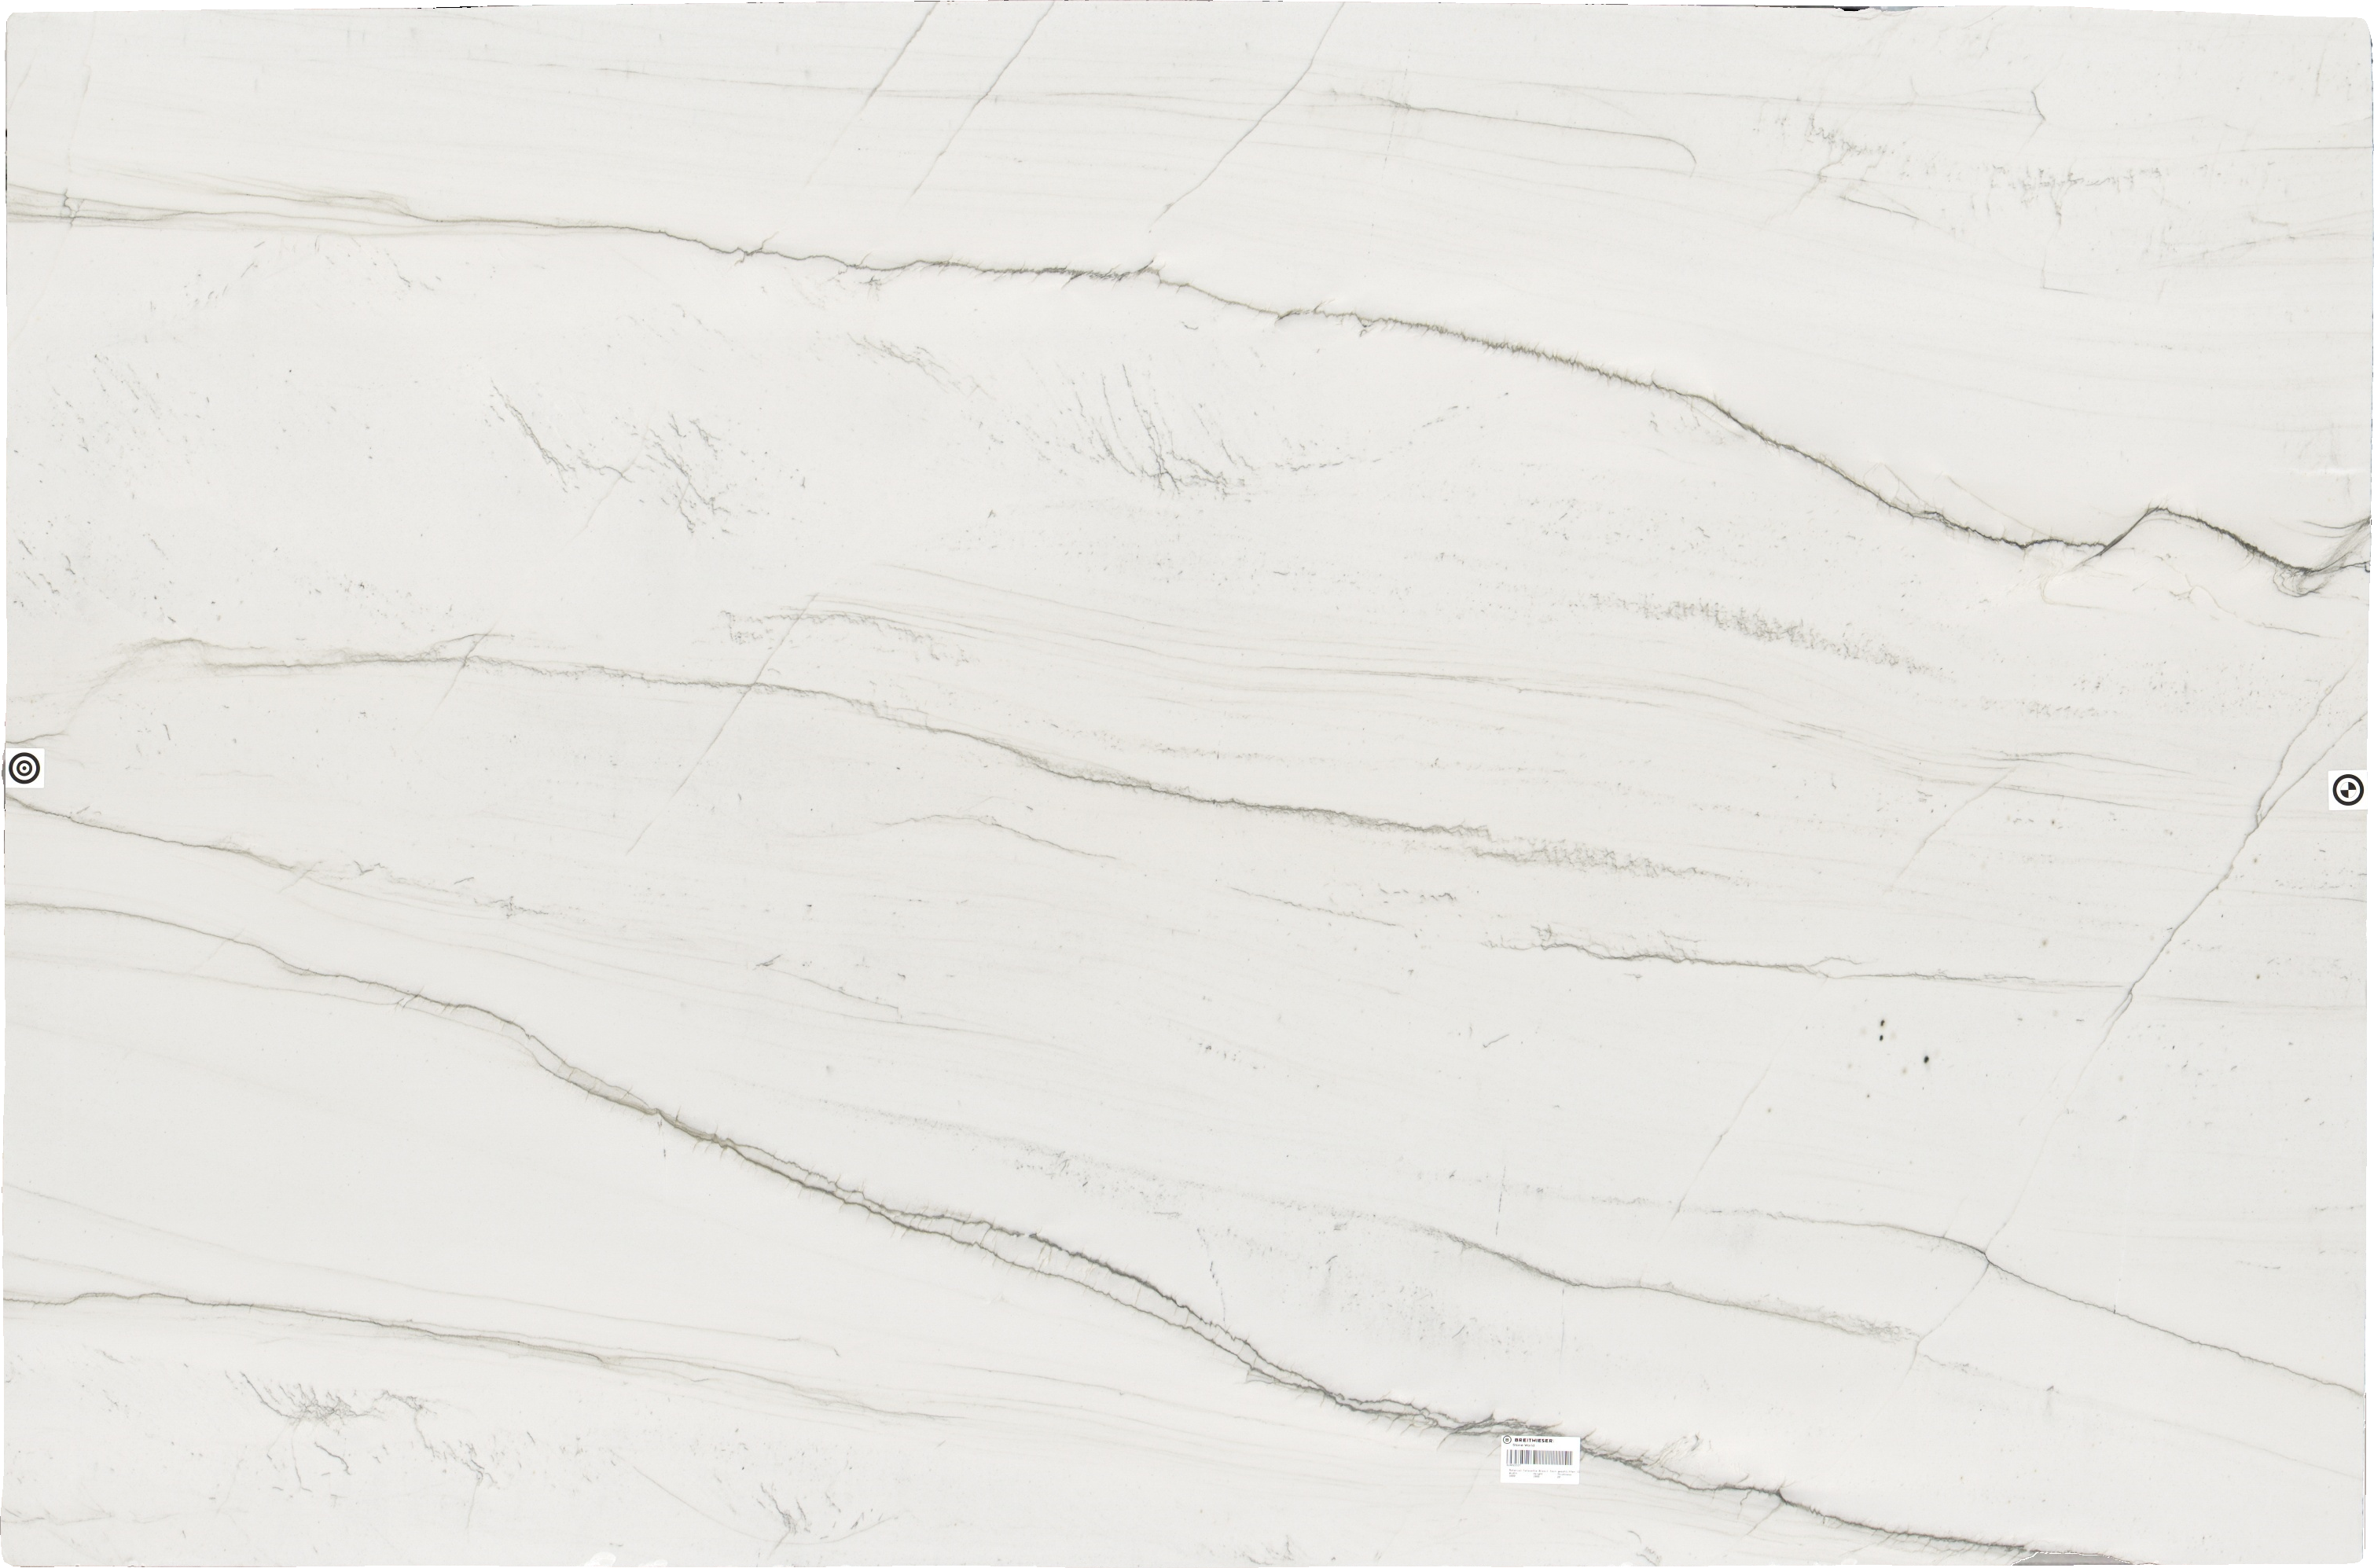
\includegraphics[width=.7\textwidth]{slabs/canny/canny_origin}
        \caption{HED}\label{fig:hed_compare}
    \end{figure}
\end{itemize}
\subsubsection{Milestone:}
At the conclusion of this period, the results indicated that the Meijering \& Contrast filter and the Canny Edge Detection methods were the most effective. 
The \gls{HEDG} method was discarded due to its sluggish performance and subpar results, often introducing noise in the form of random lines into the images. 
The two preferred methods successfully extracted the vein structures from the images, considering that an unsupervised approach was employed.
\subsubsection{Improvements:}
One potential avenue for improvement involves the utilization of a supervised method for vein extraction. 
This method would offer greater accuracy compared to unsupervised methods, as it would be trained specifically for vein extraction. 
However, implementing a supervised approach necessitates significant time and a substantial number of hand-labeled images to train the model effectively.

\subsection{Fourth Period:}
During this designated period, the focus was on training the network. 
The network employed for this purpose was a pix2pix network, which utilizes a Conditional Generative Adversarial Network (\gls{cgang}) to generate images. 
The training process involved utilizing the dataset created in the preceding periods and the hardware resources provided by the company (See~\ref{subsec:hardware})

Various configurations of the network were tested during this period, involving the fine-tuning of hyperparameters to identify the optimal setup. 
The specific configuration details of the network will be elaborated upon in Chapter~\ref{cap:design-coding}.
\subsubsection{Milestone:}
Upon the conclusion of this period, the network demonstrated its capability to generate images of slabs exhibiting a diverse range of colors and textures (See~\ref*{fig:gen-images}).
%list of img generated
\begin{figure}
    \centering
    \includegraphics[width=.7\textwidth]{slabs/generated/amogus}
    \\
    \includegraphics[width=.7\textwidth]{slabs/generated/breton}
    \\
    \includegraphics[width=.7\textwidth]{slabs/generated/slab}
    \caption{Generated images}\label{fig:gen-images}
\end{figure}
    %\input{chapters/concept}
    \chapter{Design and coding}\label{cap:design-coding}
\intro{In this chapter we will describe the design and coding of the project.
We will start by describing the technologies and tools used, then we will
describe the software life cycle, the design and the design patterns used and
finally we will describe the coding phase.}


\section{Technology and tools}\label{sec:technology-tools}
In the following sections we will describe the technologies and tools used in
the project.
\subsection*{Python}\label{subsec:python}
Python is a programming language that lets you work quickly and integrate
systems more effectively. It is a high-level programming language, with
applications in numerous areas, including web programming, scripting, scientific
computing, and artificial intelligence. It is very popular and used by many
companies, such as Google, Facebook, Instagram, Spotify, Netflix, Dropbox, and
many others. It is also used in the development of many open source projects,
such as Blender, GIMP, Inkscape, and many others. It is a very versatile
language, with a very large community and a very large number of libraries
available. It is also a very simple language to learn, with a very simple
syntax, which makes it very readable and easy to understand. It is also a
language that is constantly evolving, with new versions released every year,
which makes it always up to date and with the latest technologies.

\subsection*{CUDA}\label{subsec:cuda}
CUDA is a parallel computing platform and programming model developed by NVIDIA
for general computing on graphical processing units (GPUs). With CUDA, developers
are able to dramatically speed up computing applications by harnessing the power
of GPUs. In GPU-accelerated applications, the sequential part of the workload
runs on the CPU – which is optimized for single-threaded performance – while the
compute intensive portion of the application runs on thousands of GPU cores in
parallel. When using CUDA, developers program in popular languages such as C,
C++, Fortran, Python and MATLAB and express parallelism through extensions in
the form of a few basic keywords.

\subsection*{CuDNN}\label{subsec:cudnn}
The NVIDIA CUDA® Deep Neural Network library (cuDNN) is a GPU-accelerated library
of primitives for deep neural networks.
cuDNN provides highly tuned implementations for standard routines such as forward and backward convolution,
pooling, normalization, and activation layers. 
cuDNN is part of the NVIDIA Deep Learning SDK.\@
\subsection*{ML libraries}\label{subsec:mllib}
\subsubsection*{TensorFlow}\label{subsubsec:tensorflow}
TensorFlow is an end-to-end open source platform for machine learning. It has a
comprehensive, flexible ecosystem of tools, libraries and community resources
that lets researchers push the state-of-the-art in ML and developers easily
build and deploy ML powered applications.
\subsubsection*{PyTorch}\label{subsubsec:pytorch}
PyTorch is an open source machine learning library based on the Torch library,
used for applications such as computer vision and natural language processing,
primarily developed by Facebook's AI Research lab (FAIR). It is free and open
source software released under the Modified BSD license. Although the Python
interface is more polished and the primary focus of development, PyTorch also
has a C++ interface.
\subsubsection*{Keras}\label{subsubsec:keras}
Keras is a high-level neural networks \gls{apig}, written in Python and capable of
running on top of TensorFlow, CNTK, or Theano. It was developed with a focus on
enabling fast experimentation. Being able to go from idea to result with the
least possible delay is key to doing good research.
\subsubsection*{OpenCV}\label{subsubsec:opencv}
OpenCV (Open Source Computer Vision Library) is an open source computer vision
and machine learning software library. OpenCV was built to provide a common
infrastructure for computer vision applications and to accelerate the use of
machine perception in the commercial products. Being a BSD-licensed product,    
OpenCV makes it easy for businesses to utilize and modify the code. The library
has more than 2500 optimized algorithms, which includes a comprehensive set of
both classic and state-of-the-art computer vision and machine learning
algorithms. These algorithms can be used to detect and recognize faces, identify
objects, classify human actions in videos, track camera movements, track moving
objects, extract 3D models of objects, produce 3D point clouds from stereo
cameras, stitch images together to produce a high resolution image of an entire
scene, find similar images from an image database, remove red eyes from images
taken using flash, follow eye movements, recognize scenery and establish markers
to overlay it with augmented reality, etc. OpenCV has more than 47 thousand
people of user community and estimated number of downloads exceeding 18 million.
The library is used extensively in companies, research groups and by governmental
bodies.
\subsection*{GANs Models}\label{subsec:gans-models}
\subsubsection*{Pix2Pix}\footcite{paper:pix2pix}\label{subsubsec:pix2pix}
Pix2Pix is a Generative Adversarial Network, or \gls{gang}, model designed for general
purpose image-to-image translation. The model was trained and evaluated on a
large dataset of paired images from the \textit{Berkeley Segmentation Dataset
and Benchmark} and demonstrates a capability to generate plausible synthetic
images for a variety of image-to-image translation tasks, such as converting
daylight images to night.

\subsubsection*{ESRGAN}\footcite{paper:esrgan}\label{subsubsec:esrgan}
ESRGAN is an enhanced version of the \gls{esrgang} model, which is a Generative
Adversarial Network, or \gls{gang}, model designed for general purpose
image-to-image translation. The model was trained and evaluated on a large
dataset of paired images from the DIV2K dataset and demonstrates a capability to
generate plausible synthetic images for a variety of image-to-image translation
tasks, such as converting low resolution images to high resolution.

\subsubsection*{StyleGAN}\label{subsubsec:stylegan}
StyleGAN is a Generative Adversarial Network, or \gls{gang}, model designed for
general purpose image generation. The model was trained and evaluated on a large
dataset of unpaired images from the Flickr-Faces-HQ dataset and demonstrates a
capability to generate plausible synthetic images for a variety of image
generation tasks, such as generating realistic human faces.

\subsection*{Tools}\label{subsec:tools}
\subsubsection*{Visual Studio Code}\label{subsubsec:vscode}
Visual Studio Code is a free source-code editor made by Microsoft for Windows,
Linux and macOS.\@ Features include support for debugging, syntax highlighting,
intelligent code completion, snippets, code refactoring, and embedded Git.
\subsubsection*{Git}\label{subsubsec:git}
Git is a distributed version-control system for tracking changes in source code
during software development. It is designed for coordinating work among
programmers, but it can be used to track changes in any set of files. Its goals
include speed, data integrity, and support for distributed, non-linear
workflows.
\subsubsection*{GitHub}\label{subsubsec:github}
GitHub is a global company that provides hosting for software development
version control using Git. It is a subsidiary of Microsoft, which acquired the
company in 2018 for \$7.5 billion. It offers all of the distributed version
control and source code management (SCM) functionality of Git as well as adding
its own features. It provides access control and several collaboration features
such as bug tracking, feature requests, task management, and wikis for every
project.
\subsubsection*{GIMP}\label{subsubsec:gimp}
GIMP is a free and open-source raster graphics editor used for image retouching
and editing, free-form drawing, converting between different image formats, and
more specialized tasks.
\subsubsection*{Webex}\label{subsubsec:webex}
Webex is a video conferencing software developed by Cisco Systems. It is a
cloud-based software that provides video conferencing, online meetings,
screen-sharing, and webinars. It has a free version that allows up to 100
participants, with a 50-minute time restriction. The paid version starts at
\$13.50/month and allows up to 200 participants and unlimited meeting time.
\subsubsection*{Outlook}\label{subsubsec:outlook}
Outlook is a personal information manager software system from Microsoft,
available as a part of the Microsoft Office suite. Primarily an email
application, it also includes a calendar, task manager, contact manager,
note taking, journal, and web browsing.

\subsection*{Hardware}\label{subsec:hardware}
All the hardware used for the development of this project was provided by the
company. The hardware used for the development of this project is listed below: \\
\begin{itemize}
    \item \textbf{DELL Precision 7670}
    \begin{itemize}
        \item \textbf{CPU}: Intel Core i7-12850HX
        \item \textbf{GPU}: NVIDIA Quadro RTX A2000 8GB GDDR6
        \item \textbf{RAM}: 32GB DDR4
        \item \textbf{Storage}: 512GB NVMe SSD
        \item \textbf{OS}: Windows 10 Pro 64-bit
    \end{itemize}
    \item \textbf{DELL Precision 7520}
    \begin{itemize}
        \item \textbf{CPU}: Intel Core i7-6820HQ
        \item \textbf{GPU}: NVIDIA Quadro M2200 4GB GDDR5
        \item \textbf{RAM}: 16GB DDR4
        \item \textbf{Storage}: 512GB NVMe SSD
        \item \textbf{OS}: Windows 10 Pro 64-bit
    \end{itemize}
\end{itemize}
\section{Final implementation}\label{sec:final-implementation}
\subsection{Network Type}\label{subsec:network-type}
For the final implementation of the project, the network type chosen was the Pix2Pix model.
\subsubsection{Pix2Pix in detail}\label{subsubsec:pix2pix-in-detail}
Pix2Pix is a Generative Adversarial Network, or \gls{gang}, model designed for general purpose image-to-image translation.
The two models are build as the following:
\subsubsection{U-Net Generator}
The generator follow the U-Net architecture, which is a convolutional neural network that
consists of an encoder (down-sampler) and a decoder (up-sampler). The encoder downsamples the
input image and extracts the features, while the decoder upsamples the image and produces
the segmentation map. The skip connections between the encoder and decoder are added to
prevent the loss of low-level features during the upsampling process.
\begin{figure}[H]
    \centering
    \includegraphics[width=0.5\textwidth]{model/unet-gen}
    \caption{U-Net architecture}\label{fig:unet}
\end{figure}
\subsubsection{TensorFlow implementation}
The TensorFlow implementation of the U-Net generator is composed by the following layers (see figure~\ref{fig:gen-layer}):
\begin{itemize}
    \item \textbf{Encoder}: 8 downsampling layers, each downsampling layer is composed by a convolutional layer, a batch normalization layer, and a Leaky ReLU activation layer.
    \item \textbf{Decoder}: 8 upsampling layers, each upsampling layer is composed by a transposed convolutional layer, a batch normalization layer, a dropout layer(applied to the first 3 layers), and a ReLU activation layer.
    \item \textbf{Skip connections}: between the encoder and decoder, there are skip connections, each skip connection.
\end{itemize}
\begin{figure}[H]
    \centering
    \includegraphics[width=0.85\textwidth]{model/generator-layer}
    \caption{TensorFlow implementation of the U-Net generator}\label{fig:gen-layer}
\end{figure}
\subsection{PatchGAN Discriminator}\label{subsec:patchgan-discriminator}
The discriminator is a convolutional neural network that classifies the real and fake
images. The discriminator architecture is such that each convolutional block in the
discriminator consists of a convolution layer, a batch normalization layer, and a Leaky
ReLU activation layer. The PatchGAN discriminator architecture is such that it only penalizes
the structure at the scale of patches. This discriminator tries to classify if each N x N
patch in an image is real or fake.
\begin{figure}[H]
    \centering
    \includegraphics[width=0.6\textwidth]{model/patch-gan}
    \caption{PatchGAN discriminator.}\label{fig:patchgan}
\end{figure}
Each value of the output matrix in fig.~\ref*{fig:patchgan} represents the probability of whether the corresponding image patch is real or it is artificially generated.
\subsubsection{TensorFlow implementation}
The TensorFlow implementation of the PatchGAN discriminator is composed by the following layers (see figure~\ref{fig:dis-layer}):
\begin{itemize}
    \item \textbf{Input}: 2 input layers, one for the real image and one for the generated image.
    \item \textbf{Concatenate}: the two input layers are concatenated along the channel axis.
    \item \textbf{Downsampling}: the concatenated input is downsampled using 3 convolutional layers, each convolutional layer is composed by a convolutional layer, a batch normalization layer, and a Leaky ReLU activation layer.
    \item \textbf{Output}: the output layer is a 30$\times$30$\times$1 matrix, where each patch of the output classifies a 70$\times$70 portion of the input image as real or fake.
\end{itemize}
\begin{figure}[H]
    \centering
    \includegraphics[width=0.85\textwidth]{model/discriminator-layer}
    \caption{TensorFlow implementation of the PatchGAN discriminator}\label{fig:dis-layer}
\end{figure}
\subsection{Adam optimizer}\label{subsubsec:adam-optimizer}
The Adam optimizer is a widely used optimization algorithm for training neural networks. 
It was introduced by Diederik P. Kingma and Jimmy Ba in their paper titled ``Adam: A Method for Stochastic Optimization'~\footcite{paper:kingma2014adam} published in 2015. 
Adam stands for Adaptive Moment Estimation and combines the benefits of two other optimization techniques: AdaGrad and RMSProp. It maintains adaptive learning rates for each parameter, automatically adjusting the learning rate based on the gradient's past behavior. 
By utilizing first and second moments of the gradients, Adam updates the parameters to accelerate convergence and handle different types of neural networks effectively.
It can be used instead of the classical stochastic gradient descent procedure to update network weights iterative based on training data.
According to Kingma et al., the method is ``computationally efficient, has little memory requirements, invariant to diagonal rescaling of gradients, and is well suited for problems that are large in terms of data and/or parameters``.
\par
Following the pix2pix paper, the Adam optimizer is used with a learning rate of 0.0002 and momentum of 0.5 for both the generator and the discriminator.
\subsection{Training process}\label{subsec:training-process}
For the generator training the procedure is the following illustrated in fig.~\ref{fig:gen-training}, Meanwhile for the discriminator training the procedure is the following illustrated in fig.~\ref{fig:dis-training}.
\par
The training process begins with pairs of input images and their corresponding target output images. 
The generator network takes the input image as input and generates a synthesized output image. 
The discriminator network, on the other hand, receives both the synthesized output image from the generator and the real target output image. 
The discriminator's objective is to correctly classify whether the input image is real or synthesized.
\par
The training process involves alternating between two steps: generator update and discriminator update. 
In the generator update step, the generator parameters are updated to minimize the discrepancy between the synthesized output image and the target output image. 
This is typically done by minimizing a pixel-wise loss function, such as mean squared error or binary cross-entropy, which measures the difference between the synthesized and target images.
\par 
In the discriminator update step, the discriminator parameters are updated to improve its ability to discriminate between real and synthesized images. 
The discriminator is trained to correctly classify real images as real and synthesized images as fake. It aims to maximize its classification accuracy.
\par
The training process continues iteratively, with the generator and discriminator networks playing a competitive game. 
The generator learns to generate more realistic and visually appealing output images that closely resemble the target images, while the discriminator becomes more skilled at distinguishing between real and synthesized images.
\par
This adversarial training process creates a feedback loop where the generator tries to produce images that the discriminator cannot distinguish from real ones, and the discriminator continuously improves its ability to discriminate between real and synthesized images. 
This iterative training process helps the generator network learn to generate high-quality output images that are visually consistent with the target images.
\par
The training process of the pix2pix generator and discriminator involves this iterative interplay, gradually improving the generator's ability to synthesize realistic output images and the discriminator's ability to distinguish between real and synthesized images.
\begin{figure}
    \centering
    \includegraphics[width=0.50\textwidth]{model/gen-training}
    \caption{Generator training process}\label{fig:gen-training}
    \includegraphics[width=0.50\textwidth]{model/dis-training}
    \caption{Discriminator training process}\label{fig:dis-training}
\end{figure}
\subsection{User Interface}\label{subsec:user-interface}
As a requirements of the project, a user interface was developed to allow the user to draw the input image.
It was developed using the Python library Tkinter and it is composed by a window with a menu bar and a canvas where the user can draw.
The menu bar consists of the following:
\begin{itemize}
    \item \textbf{Colors}
    \begin{itemize}
        \item \textbf{Brush Color}: Set the Brush color.
        \item \textbf{background Color}: Set the background color.
    \end{itemize}
    \item \textbf{Options}
    \begin{itemize}
        \item \textbf{Clear canvas}: Undo the last action.
        \item \textbf{Generate Image}: Redo the last action.
        \item \textbf{Load CAD}: Load a CAD file as input.
        \item \textbf{Load PNG/JPG}: Load a .PNG file as input.
        \item \textbf{Exit}: Exit the application.
    \end{itemize}
\end{itemize}
\begin{figure}[H]
    \centering
    \includegraphics[width=0.50\textwidth]{ui/ui}
    \caption{User interface}\label{fig:ui}
\end{figure}
Once the input is submitted, the application will show the output in the lower canvas.
And save it in the \textit{output} folder.

    \chapter{Verification and validation}\label{cap:verification-validation}
\intro{
    In this chapter we will discuss the verification and validation process of the trained model.
    We will discuss the metrics used to evaluate the model and the results obtained.
}
\section{Metrics}\label{sec:metrics}
\subsection{Loss function}
According to the pix2pix paper \footcite{paper:pix2pix}, the loss function used is a combination of a conditional GAN loss and a L1 loss.
In a general CGAN the objective function is defined as:
\begin{equation}
    \label{eq:cgan-loss}
    L_{cGAN}(G, D) = \mathbb{E}_{x,y}[\log D(x, y)] + \mathbb{E}_{x,z}[\log(1 - D(x, G(x, z)))]
\end{equation}
here $G$ tries to minimize this function against an adversarial $D$ that tries to maximize it.
To assess the significance of conditioning the discriminator, we also compare it to an unconditional variant where the discriminator does not have access to the input x. 
The loss function for this unconditional variant can be expressed as:
\begin{equation}
    \label{eq:cgan-loss-uncond}
    L_{cGAN}(G, D) = \mathbb{E}_{x,y}[\log D(y)] + \mathbb{E}_{x,z}[\log(1 - D(G(x, z)))]
\end{equation}
Previous studies have shown the advantages of incorporating a traditional loss, such as L2 distance \footcite{paper:DPathakCVPR16}, alongside the GAN objective. 
While the discriminator's role remains unchanged, the generator is not only responsible for fooling the discriminator but also for producing outputs that closely resemble the ground truth in terms of L2 similarity. 
Additionally, we explore an alternative option by employing L1 distance instead of L2, as L1 promotes reduced blurring:
The L1 loss for the generator can be defined as:
\begin{equation}
    \label{eq:l1-loss}
    L_{L1}(G) = \mathbb{E}_{x,y,z}\left[\left\|y - G(x, z)\right\|_1\right]
\end{equation}
Our ultimate objective is to find the optimal generator G that minimizes the loss function while simultaneously maximizing the performance of the discriminator D. 
This objective can be represented by the equation:
\begin{equation}
    G^* = \arg \min_G \max_D \left( L_{cGAN}(G, D) + \lambda L_{L1}(G) \right)
\end{equation}
In previous conditional GAN approaches, the inclusion of Gaussian noise z alongside the input x was employed to prevent deterministic outputs and allow for the modeling of diverse distributions. 
However, in our experiments, this strategy was found to be ineffective as the generator learned to ignore the noise, aligning with the findings of Mathieu et al. \footcite{paper:MMathieuICLR16}. 
Instead, in our final models, we introduce noise through the use of dropout applied to multiple layers of the generator during both training and testing. 
Despite the presence of dropout noise, we observe only minor stochasticity in the generated outputs. 
The development of conditional GANs that can produce highly stochastic outputs, capturing the full entropy of the conditional distributions they model, remains an open and important question for future research.
%\subsection{Evaluation metrics}
%\subsubsection{\gls{fidg} score}
%The Fréchet Inception Distance (\gls{fidg}\glsfirstoccur) score is a widely used metric for evaluating the quality of generated images in the field of generative adversarial networks (GANs) introduced by Martin Heusel et al. \footcite{paper:heusel2017gans}. 
%It measures the similarity between the distribution of real images and the distribution of generated images by comparing their feature representations extracted from a pre-trained Inception-v3 network. 
%A lower FID score indicates better similarity between the two distributions, suggesting higher-quality generated images that resemble the real data more closely. 
%The FID score takes into account both the quality and diversity of generated images, making it a valuable metric for assessing the performance of GAN models. 
%It provides a quantitative measure that complements visual inspection and subjective evaluation, enabling researchers to objectively compare and analyze different GAN architectures and training strategies.
%The \gls{fidg} score is defined as:
%\begin{equation}
%    \label{eq:fid-score}
%    \text{FID}(p, q) = \|\mu_p - \mu_q\|^2 + \text{Tr}(\Sigma_p + \Sigma_q - 2(\Sigma_p\Sigma_q)^{1/2})
%\end{equation}
%Where:
%\begin{itemize}
%    \item $\mu_p$ and $\mu_q$ are the mean vectors of the real and generated images respectively.
%    \item $\Sigma_p$ and $\Sigma_q$ are the covariance matrices of the real and generated images respectively.
%    \item \text{Tr} is the trace operator.
%    \item $\|\cdot\|$ is the Euclidean norm.
%\end{itemize}
%\subsubsection{Inception score}

\section{Results}\label{sec:results}
\subsection{Evaluation metrics}
During the training process, the evaluation metrics were calculated every 100 epochs.
For get a more accurate result, the evaluation metrics were calculated using the same couple of image-mask for each epoch, generating ten images for each epoch.
Each generated image was compared with the corresponding real image.
\subsubsection{FID score}
During the training process, the FID score was calculated every 100 epochs. 
%Table for compare FID score
\begin{table}[H]
    \centering
    \begin{tabular}{|c|c|c|}
        \hline
        \textbf{Model} & \textbf{FID score} & \textbf{Epoch} \\
        \hline
        \hline
        \textbf{M1} & 32,98 & 100 \\
        \hline
        \textbf{M2} & 26,42 & 200 \\
        \hline
        \textbf{M3} & 25,39 & 300 \\
        \hline
        \textbf{M4} & 22,29 & 400 \\
        \hline
        \textbf{M5} & 22,29 & 500 \\
        \hline
        \textbf{M6} & 22,29 & 600 \\
    \end{tabular}
    \caption{Mean FID score for each model}\label{tab:fid-score}
\end{table}
According to the results obtained, the best model is the \textbf{M3} model.
\subsubsection{Inception score}
During the training process, the Inception score was calculated every 100 epochs.
%Table for compare Inception score
\begin{table}[H]
    \centering
    \begin{tabular}{|c|c|c|}
        \hline
        \textbf{Model} & \textbf{Inception score} & \textbf{Epoch} \\
        \hline
        \hline
        \textbf{M1} & 0,6589 & 100 \\
        \hline
        \textbf{M2} & 0,7461 & 200 \\
        \hline
        \textbf{M3} & 0,7596 & 300 \\
        \hline
        \textbf{M4} & 0,7435 & 400 \\
        \hline
        \textbf{M5} & 0,7005 & 500 \\
        \hline
        \textbf{M6} & 0,7362 & 600 \\
    \end{tabular}
    \caption{Mean Inception score for each model}\label{tab:inception-score}
\end{table}
According to the results obtained, the best model is the \textbf{M3} model.

\section{Different Network Configurations}\label{sec:different-network-configurations}
During the training process, a problem was encountered where the image quality started to deteriorate after a certain number of epochs. Upon analyzing the loss curve, it became evident that the discriminator's loss was decreasing rapidly. 
This led me to believe that the discriminator was learning features at a faster rate than the generator.
To address this issue, I made several adjustments to the network's hyper-parameters:
\begin{itemize}
    \item Initially, I started training with the standard configuration and disabled discriminator training after 140k steps to prevent it from surpassing the generator's performance. Unfortunately, this modification resulted in even worse outcomes.
    \item I also experimented with disabling dropout on the three layers, suspecting that it might be responsible for the poor results and adversely affecting the model.
    \item Another attempt involved training the model for 150k steps and reducing the discriminator's learning rate to 0.0001, instead of completely disabling its training. However, this approach also yielded unsatisfactory results.
\end{itemize}
Ultimately, it was discovered that the issue did not lie with the network's hyper-parameters, but rather with the training dataset itself.
The training dataset posed a challenge as it was created through an unsupervised process, resulting in the inclusion of numerous low-quality images. Some of these images contained only white spots instead of a complete line representing a vein, which affected the overall image quality. Recognizing this issue, I took steps to address it by removing such problematic images from the dataset.

As the training progressed and these flawed images were eliminated, the image quality gradually improved with each epoch. This suggests that the removal of these specific images played a crucial role in enhancing the overall performance and realism of the generated images.
    \chapter{Conclusion}
\label{cap:conclusioni}

\section{Consuntivo finale}

\section{Raggiungimento degli obiettivi}

\section{Conoscenze acquisite}

\section{Valutazione personale}


    %\appendix
    %\chapter{Appendix A}

\epigraph{Citazione}{Autore della citazione}


    \backmatter
    \printglossary[type=\acronymtype, title=Acronyms and abbreviations, toctitle=Acronyms and abbreviations]
    \printglossary[type=main, title=Glossary, toctitle=Glossary]

    \cleardoublepage\chapter{Bibliography}
\nocite{*}
% Print book bibliography
\printbibliography[heading=subbibliography,title={Book bibliography},type=book]
% Print site bibliography
\printbibliography[heading=subbibliography,title={Web-Site bibliography},type=online]
% Print article bibliography
\printbibliography[heading=subbibliography,title={Article bibliography},type=article]

\end{document}
